\stfhIndex{I156}{Shouyaozhangai}{首要障碍（primary obstruction）}
\section{\termPrimaryObstruction{}与全纯圆盘}
\label{sec:primary-obstruction-holomorphic-discs}

本节尝试从紧拉格朗日子流形的对子 $(L_0,L_1)$（其中 $L_0\pitchfork L_1$）中提取
第 13.8 节所表述的抽象\personFloer{}复形结构，并说明不同于闭弦情形，\termAnomaly{}如何在这种开弦
情形中出现。

设 $(L_0,L_1)$ 是\termTransversePair{}。记
\[
 \operatorname{Int}(L_0,L_1;\ell_0)
 =\{x\in L_0\cap L_1\mid \ell_x\text{ 位于 }\Omega(L_0,L_1;\ell_0)\},
\]
以及
\[
 CF(L_0,L_1;\ell_0)
 =\operatorname{Int}(L_0,L_1;\ell_0)\text{ 上的自由 }
 \Lambda(L_0,L_1;\ell_0)\text{-模}.
\]

\stfhIndex{I037}{Wufanchang}{无反常（anomaly-free）}
\stfhIndex{I188}{Wuzhangai}{无障碍（unobstructed）}
\begin{definition}
\label{def:anomaly-free-pair}
若 $(L_0,L_1)$ 配有满足下列条件的 $J=\{J_t\}$，则称它是\emph{\termAnomalyFree{}的}或
\emph{\termUnobstructed{}的}。
\begin{enumerate}[label=(\arabic*)]
\item 对任意满足
\[
 \mu(x,y;B)\leq0
\]
的对子 $\{x,y\}\subset\operatorname{Int}(L_0,L_1;\ell_0)$，除非 $x=y$ 且
$B=0\in\pi_2(x,y)$，否则 $\widetilde{\mathcal M}(x,y;B)=\varnothing$。当
$x=y$ 且 $B=0$ 时，解只有\termStationarySolution{}，即对所有 $\tau\in\mathbb R$ 都有
$u(\tau)\equiv x=y$。
\item 对任意 $\{x,y\}\subset\operatorname{Int}(L_0,L_1;\ell_0)$ 和满足
$\mu(x,y;B)=1$ 的同伦类 $B\in\pi_2(x,y)$，
\[
 \mathcal M(x,y;B)=\widetilde{\mathcal M}(x,y;B)/\mathbb R
\]
是\personFredholm{}正则且紧的，因而是有限集。记
\[
 n(x,y;B)=\#\mathcal M(x,y;B)
\]
为 $\mathcal M(x,y;B)$ 中元素的代数计数；其他情况下令 $n(x,y;B)=0$。
\item 对任意 $\{x,y\}\subset\operatorname{Int}(L_0,L_1;\ell_0)$ 和满足
$\mu(x,y;B)=2$ 的 $B\in\pi_2(x,y)$，$\mathcal M(x,y;B)$ 可以紧化为一个光滑
一维流形，它或者无边界，或者其边界由断裂流线
\[
 u_1\#_\infty u_2
\]
组成；这里遍历所有可能的 $y\in\operatorname{Int}(L_0,L_1;\ell_0)$ 以及
$B_1\in\pi_2(x,y)$、$B_2\in\pi_2(y,z)$，满足
\[
 B_1\#B_2=B,\qquad
 u_1\in\mathcal M(x,y;B_1),\qquad [u_2]\in\mathcal M(y,z;B_2),
\]
并且
\[
\mu(x,y;B_1)=\mu(y,z;B_2)=1.
\]
\footnote{译者注：原书本项开头只量化对子 $\{x,y\}$，随后却以 $u_1$ 连接
$x,y$、以 $u_2$ 连接 $y,z$，又写“遍历所有可能的 $y$”；端点变量的量化与复用
并不一致。译文照录。}
\end{enumerate}
\end{definition}

\stfhIndex{I089}{Fuluoerzhengze}{弗洛尔正则（Floer regular）}
我们称任何这样的
$J\in\mathfrak j_\omega=C^\infty([0,1],\mathcal J_\omega)$ 是
$(L_0,L_1)$-正则的，并称任何这样的三元组 $(L_0,L_1;J)$ 是\emph{\termFloerRegular{}}的。
定义中的主要假设涉及 $\mathcal M(L_0,L_1;J)$ 的零维分支（对应 (2)）与一维分支
（对应 (3)）的若干紧性性质。要在环 $\Lambda(L_0,L_1;\ell_0)$ 上定义复形，另一
要点是模空间上存在相容定向。为此，我们要求对子 $(L_0,L_1)$ 在 (FOOO09) 的意义下
\emph{相对 spin}。记
\[
 \mathfrak j^{\mathrm{reg}}_{(L_0,L_1)}\subset\mathfrak j_\omega
\]
为所有 $(L_0,L_1)$-正则 $J$ 的集合。对任意给定的横截相交对子 $(L_0,L_1)$，
$\mathfrak j^{\mathrm{reg}}_{(L_0,L_1)}$ 在 $\mathfrak j_\omega$ 中稠密。

\stfhIndex{I132}{Dandiaolagelangriziliuxing}{单调拉格朗日子流形（monotone Lagrangian submanifold）}
这里要指出，在正合情形之外，如此强意义下的\termUnobstructed{}对子相当少见。不过，(Oh93a)
挑出了一类特殊的\termUnobstructed{}对子，即\emph{单调}拉格朗日子流形 $L$ 的对子；它在一般拉格朗日\personFloer{}理论的发展中起着重要作用。

我们先考察取自 (Oh93b)、(FOOO09) 的简单例子，它展示了使\personFloer{}边界映射的边界
性质发生\termAnomaly{}的“\termInstantonEffects{}”。

\begin{example}
\label{ex:disc-bubble-anomaly-plane}
考虑 $(M,\omega)=(\mathbb C,\omega_0)$ 以及
\[
 L_0=\mathbb R+\sqrt{-1}\cdot0,\qquad L_1=S^1=\partial D^2(1).
\]
$L_0$ 与 $M$ 都不紧。不过，可以把 $\mathbb C$ 共形紧化为
$\mathbb P^1\cong S^2$，使 $\mathbb R$ 与 $S^1$ 都成为赤道。$L_0$ 与 $L_1$ 交于
两点，记为
\[
 p=(-1,0),\qquad q=(1,0).
\]
考察模空间 $\mathcal M(p,q)$、$\mathcal M(q,p)$ 与 $\mathcal M(p,p)$。容易看出，
$\pi_2(p,q)=\pi_2(L_0,L_1;p,q)$ 是 $\pi_2(\mathbb C,S^1)\cong\pi_1(S^1)$ 的\termTorsor{}。以 $B_1\in\pi_2(p,q)$ 表示由显然的上半圆盘所代表的同伦类；类似地，
以 $B_2\in\pi_2(q,p)$ 表示由下半圆盘代表的类。再令 $B\in\pi_2(p,p)$ 为
\[
 B=B_1\#B_2.
\]
马斯洛夫指标计算给出
\[
 \mu(p,q;B_1)=\mu(q,p;B_2)=1,
\]
故 $\mu(p,p;B)=2$。

\begin{figure}[htbp]
 \centering
 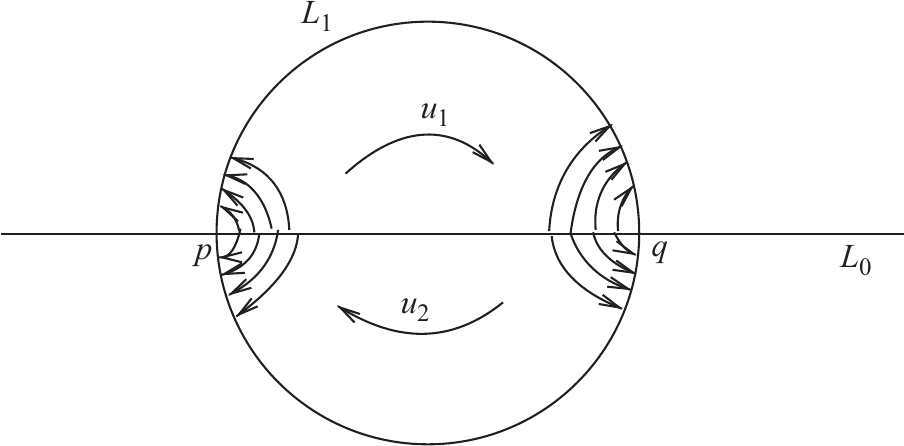
\includegraphics[width=.62\textwidth]{chapters/ch16-monotone-lagrangian-floer/figures/figure-16-1.png}
 \caption{全纯映射 $u_1,u_2$。}
 \label{fig:holomorphic-maps-u1-u2}
\end{figure}

由带边界的\personRiemann{}映射定理的简单应用可知，$\mathcal M(p,q;B_1)$ 恰有一个元素，
它由 $u_1:\mathbb R\times[0,1]\to\mathbb C$ 代表，其像为显然的上半圆盘（图
\ref{fig:holomorphic-maps-u1-u2}）。类似地，$\mathcal M(q,p;B_2)$ 恰有一个元素，
其像为下半圆盘。再对\personRiemann{}--\personHilbert{}问题作简单线性分析，还可证明这些映射正则，
即其线性化映射满射。由维数考察得到
\[
 \partial([\ell_p,w])=[q,w\#B_1],
 \qquad
 \partial([\ell_q,w'])=[p,w'\#B_2],
\]
其中 $w,w'$ 分别遍历 $\ell_p,\ell_q$ 的\termBoundingDisc{}。
\end{example}

\begin{exercise}
\label{ex:prove-plane-boundary-formula}
证明上述断言。
\end{exercise}

现在分析 $\mathcal M(p,p;B)$。把 $\mathcal M(p,p;B)$ 的每个元素视为对应于
$\widetilde{\mathcal M}(p,p;B)$ 中元素的无参数化曲线，由\personRiemann{}映射定理可证，
它由 $-1<\ell<1$ 时的全纯映射 $u_\ell:\mathbb R\times[0,1]\to\mathbb C$
组成，并满足
\[
 \begin{gathered}
 u_\ell(\mathbb R\times\{0\})\subset\mathbb R\times\{0\},\qquad
 u_\ell(\mathbb R\times\{1\})\subset\partial D^2,\qquad [u_\ell]=B,\\
 u_\ell(-\infty,\cdot)=u_\ell(\infty,\cdot)=\ell_p,\qquad
 u_\ell(0,0)=(\ell,0).
 \end{gathered}
\]
由对称性，$u_\ell$ 还必满足 $u_\ell(0,1)=(1,0)$。可以证明，上述族确实给出
$\mathcal M(p,p;B)$ 的全部元素，并且所有映射都是\personFredholm{}正则的。由此描述，
$\mathcal M(p,p;B)$ 的一个自然紧化是在 $\ell\to1$ 的一端添入断裂流线
$u_1\#u_2$，并添入 $\ell\to-1$ 时的另一端。

\begin{figure}[htbp]
 \centering
 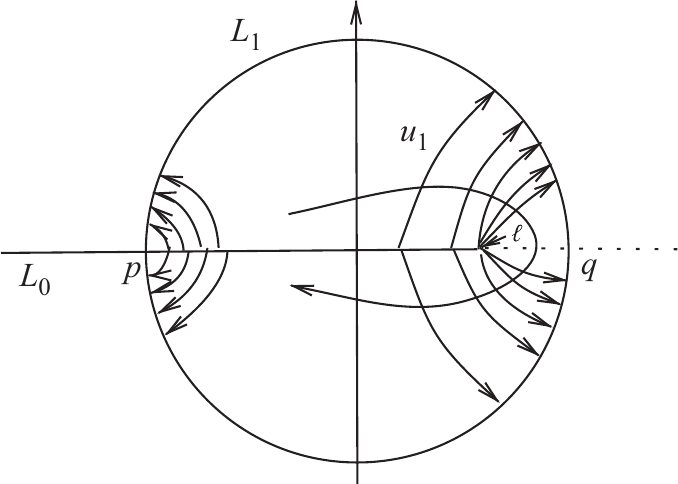
\includegraphics[width=.58\textwidth]{chapters/ch16-monotone-lagrangian-floer/figures/figure-16-2.png}
 \caption{全纯映射 $u_\ell$。}
 \label{fig:holomorphic-maps-ul}
\end{figure}

见图\ref{fig:holomorphic-maps-ul}。注意 $u_\ell$ 满足：
\begin{enumerate}[label=(\arabic*)]
\item $u_\ell(\mathbb R\times\{0\})\subset\{(t,0)\mid-1<t\leq\ell\}$；特别地，
当 $\ell\to-1$ 时，$u_\ell|_{\mathbb R\times\{0\}}$ 收敛到常值映射 $(-1,0)$；
\item $u_\ell|_{\mathbb R\times\{1\}}$ 的像恰好绕边界 $\partial D^2$ 一周。
\end{enumerate}
还可以验证，对任意紧子集
$K\subset\mathbb R\times[0,1]\setminus\{(0,1)\}$，
\[
 \|du_\ell\|_{\infty,K}\longrightarrow0\quad(\ell\to-1),
\]
同时还有
\[
 |du_\ell(0,1)|\nearrow\infty.
\]

由此分析可知，当 $\ell\to-1$ 时，上图背后的真实情形是出现了与如下奇异曲线
对应的\emph{稳定}流线：
\[
 (u_\infty,\mathbb R\times[0,1],\{(0,1)\})
 \cup(w,D^2,\{\mathrm{pt}\}).
\]
这里 $(u_\infty,\mathbb R\times[0,1],(0,1))$ 是主分支，
$u_\infty:\mathbb R\times[0,1]\to\mathbb C$ 是取常值
$p=(-1,0)$ 的映射，其定义域满足
\[
 (\mathbb R\times[0,1],\{(0,1)\})
 \cong(D^2\setminus\{\pm1\},\{\sqrt{-1}\}),
\]
而 $w:(D^2,\partial D^2)\to(\mathbb C,L_1)$ 是显然的包含映射，其定义域为边界
$\partial D^2$ 上带一个标记点的圆盘 $D^2$。

这个位形是一条可容许的稳定流线：$u_\infty$ 的定义域在边界上有三个特殊点，故它
稳定；$w$ 是非常值映射，故也稳定，因而两个映射的自同构群都平凡。对
$\mathcal M(p,p;B)$ 的上述分析计算出矩阵元
\[
 \bigl\langle(\partial\circ\partial)([\ell_p,w]),[\ell_p,w\#B]\bigr\rangle=1
\]
以及
\[
 \bigl\langle(\partial\circ\partial)([\ell_p,w]),[\ell_p,w\#B']\bigr\rangle=0
\]
（对任意 $B'\in\pi_2(p,p)$ 且 $B'\neq B$）。这清楚表明
$\partial\circ\partial\neq0$。

这个例子说明，当 $\mu(B)=2$ 时，$\mathcal M(p,p;B)$ 的边界可以含有并非断裂流线
类型的分支。还要注意，\emph{上述圆盘 $w$ 的马斯洛夫指标为 $2$}；稍后我们将看到，这并非
巧合。

事实上，对无边界紧\personRiemann{}曲面中的嵌入拉格朗日子流形而言，上述障碍是定义\personFloer{}同调的唯一障碍。在曲面上，每个一维子流形都是拉格朗日的，故紧嵌入拉格朗日子流形
是嵌入圆周的有限不交并。下面的曲面一般定理概括了这一讨论。

\begin{theorem}
\label{thm:surface-unobstructed-floer}
设 $\Sigma$ 是带面积形式的定向紧曲面。以 $\mathcal E_\Sigma^{\mathrm{ad}}$ 表示所有
连通分支都非零伦的嵌入拉格朗日子流形之集合。则对任意
$L_1,L_2\in\mathcal E_\Sigma^{\mathrm{ad}}$，取适当的\personNovikov{}环后，\personFloer{}同调
$HF(L_1,L_2;\Lambda)$ 有良定义。
\end{theorem}

在此意义下给出如下定义。

\stfhSubIndex{I189}{Wuzhangai}{无障碍（unobstructed）}{Qianruquxiandewuzhangaixing}{嵌入曲线的无障碍性（of embedded curves）}
\begin{definition}
\label{def:unobstructed-curve-surface}
设 $\Sigma$ 是带面积形式的定向紧曲面。若嵌入曲线 $\gamma\subset\Sigma$（不必连通）
没有零伦的连通分支，则称它是\termUnobstructed{}的。
\end{definition}

这是 (FOOO09) 所引入定义在二维曲面上的拉格朗日子流形情形之特例。关于高亏格曲面\termFukayaCategory{}的详细研究，可参见 (Ab08)；其中\personAbouzaid{}计算了 $\Sigma$ 上导出\personFukaya{}范畴的\personGrothendieck{}群。
